\chapter{Implementation\label{cha:chapter5}}

This chapter describes the concrete implementation of common aspects of the proposed framework as well as individual domain specific implementation. The in the concept, see \ref{cha:chapter4}, described introduction of libraries to enable an simple and adaptable solution are applied on the common aspects. The domain specific implementations provide an evidence about the generalization of the common elements as well as the applicability of the entire framework to specific domain. This chapter also compares technologies as basis of the framework. 

\section{Environment and underlying frameworks\label{sec:env}}

\subsection{Container framework}

Under the consideration of the outlined concept, especially the pipeline approach, the best fitting container framework is chosen from the family of stream processing frameworks. This enables a continuous delivery of processed data, ships with features enabling processing guarantees and mainly contributing a stable environment a feature extraction framework can build on. 
\\\\
Consequently the following alternatives must be considered as container framework:
\begin{itemize}
\item Native stream processing engine of high level programming language
\item Distributed stream and data processing framework
\item 3rd party stream processing framework
\end{itemize}

\noindent\textbf{Native stream processing engine of high level programming language:}

\noindent High level programming languages like Java already provide a library for processing data as a stream. The offer the basic data processing functions like \textit{map(.)}, \textit{fold(.)} or \textit{filter(.)}. The barrier of applying a native stream processing framework is compared to external libraries relatively low as the nature of the language is preserved. Another benefit from using such a library are compatibility issues and external dependencies. It is to favor to reduce maintenance overhead of software by reducing the number of dependencies. 

The main drawback of internal processing engines is often that the connectivity to data sources and data sinks is limited. For example do Java streams only provide a connector to files in a local file system. As the overall goal of the proposed framework is the unification of data across several sources native stream processing engines can not be considered in this concrete implementation.
\\\\
\textbf{Distributed stream and data processing framework:}

\noindent In section \ref{sec:containerframework} we already spoke about the trend of distributed data processing frameworks. Framework like Apache Flink, or Kafak Streams are specialized on data processing and provide a solid environment of features required for the proposed framework. Especially the aspect of distributed processing seems interesting when it comes to big amounts of data. Such framework minimize the implementation overhead of distributed memory management and network communication. They as well provide a brought set of adapters to different data sources and sinks. For example Apache Flink lists XY connectors. 

A minor drawback is the dependency on external developers. Every introduced program code can in the worst case contain bugs. Restrictions regarding features are set by external developers and their overall focus and road map of the library or framework. A more significant disadvantage is that this frameworks are designed to run on a distributed, clustered system. Some of the framework do in fact provide a local execution mode, but this is often only recommended for development purposes but not for production environment. Not only for the sake of simplicity also to minimize the the complexity of the system it is necessary to find a framework that allows single node deployment. It is also to mention, that throughput is not listed as a requirement for the feature extraction framework. It is also not to forget, that the frameworks concept is designed in such a ways, that it does not depend on the underlying data processing framework.
\\\\

\textbf{3rd party single node stream processing framework:}

\noindent From the previous two analysis it is to learn, that a 3rd party stream processing engine is a desirable ways to go. The requirement for reducing implementation complexity of a showcase example brings the demand for the possibility of single node deployment. Unfortunately the list of frameworks satisfying the restrictions above is short. The from the founder of the Scala programming language developed Akka framework for actors\footnote{A Actors model is a mathematical model enabling parallel and concurrent data processing.} enjoys a brought acceptance among developers. This framework provides a streaming framework on top of Akkas actor model. Akka streaming has excellent support through the close relation to the Scala programming language as well as a wide community support. Concerning the adaptivity of heterogeneous sources a community is established that provides connectors to more than 20 data sources, sinks, protocols and libraries. The alpakka library contains among others connectors to the major database systems like MongoDB, Hbase or Cassandra, as well as to file formats as CSV, XML or text files. The repertoire also lists transfer protocols like FTP, which can be beneficial for integrating remote sources of customers on a file basis.
\\\\
For the proof of concept implementation of the automation framework Akka streams is chosen as the container framework. 

\subsection{Data transfer layer}
To maintain the concept of modularization and pluggable of the framework while using Akka streams it is essential to introduce a data transfer component. Singular components realized in Akka streams need to be connected through that data transfer layer. This component is also used for the realization of the error pipeline as described in section \ref{sec:errorpipeline}. An easy to use candidate for such an application is Kafka. The streaming platform works on a publish-subscriber pattern and is a fault tolerant system for connection different software components. The ability to create different streams, named topics, comes beneficial for the error pipeline. Here each step can define its own topic to which faulty data can be published.

\subsection{Programming language and libraries}
The choice of the target programming language primarily depends on the application use case. Data processing, data transformation are often non-side-effecting applications of functions on single information entities. This can be seen in the applicability of the concept of user defined functions in the proposed framework. This leads to the conclusion that a functional programming language is well suited for this thesis' implementation. 

A second, very related aspect, is the API of the underlying framework. As the underlying framework is chosen by the best fit for the thesis' use case it is natural to imply that the underlying frameworks language is the right fit. 

This brings us to the conclusion, that the Scala programming language is a perfect candidate for a example implementation of the framework and development of the demonstrative use case.

\subsection{Internal data format}
The use of the data transfer layer urges the use of an internal data format. This aspect is already described in section \ref{sec:overalldesign}. Apache Kafka does not restrict the usage of certain data formats. Due the wide usage and human readability JSON is considered as a suitable internal data format. This also enables manual inspection of information entities on quality assurance tasks. 

\section{Implementation of input adapter and raw formats}

The implementation of the input adapter on defined library level boils down to three main classes. A data loader, a data sink and a third component to wire up the former classes. 

\subsection{Implementation of the loader component \label{ssec:loadercomponent}}

A data source specific data loader is a sub-class of the abstract generic class \textit{AbstractLoader}, compare the class diagram in figure \ref{fig:importer-diagram}, and is meant to hide the actual format of the data source as well as to transform a source element of type \textit{IN} to raw type \textit{OUT}. A \textit{AbstractLoader} requires the implementation of the data source, which is defined as a \textit{Source}-object in the Akka stream framework and can be used from the previously name Alpakka library. The abstract function \textit{tryParseElement($\cdot$)} is a function sub for the actual UDF that enables the mapping of the source schema of type \textit{IN} to the raw schema of type \textit{OUT}. The function \textit{handleFailed($\cdot$)} is called before an faulty element is written to the corresponding message queue in Kafka and can be overwritten in the case the user wants to introduce custom error handling.

As a concrete example a MongoDB loader was implemented and provided to the import adapter library for generic usage. This example utilizes the ReactiveMongo driver which is used to implement the Akka stream source as the class \textit{AbstractLoader} requires.

\begin{figure}[htb]
  \centering
  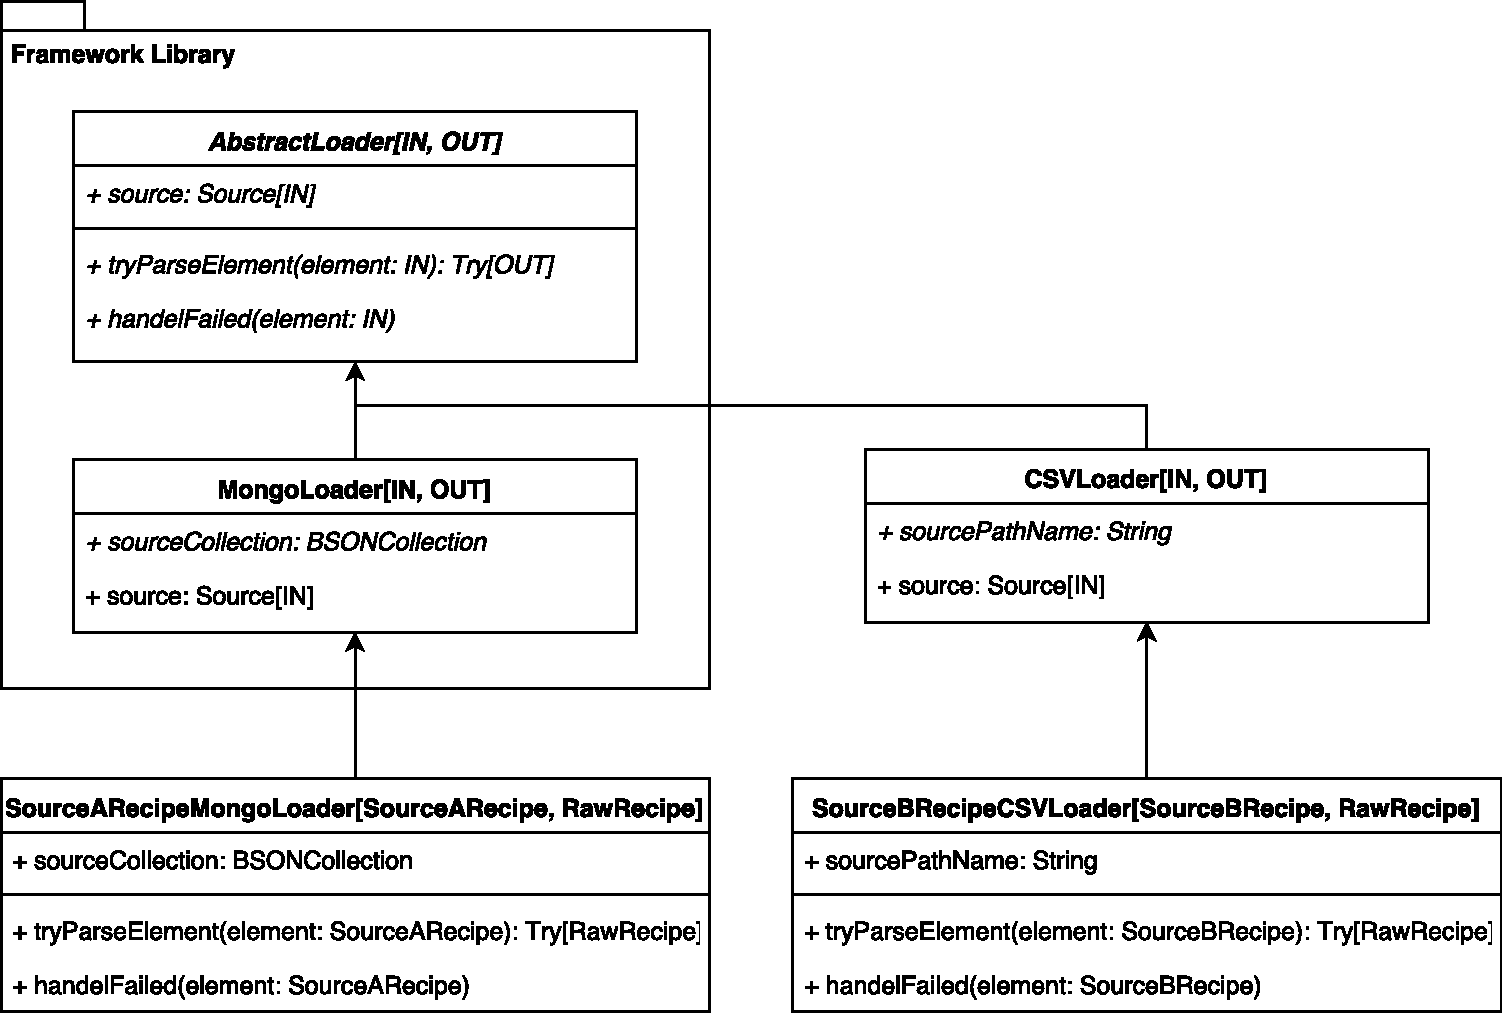
\includegraphics[width=0.9\textwidth]{importer-diagram}\\
  \caption{Class diagram of data loader library and implementation}
  \label{fig:importer-diagram}
\end{figure}

In the third level of the inheritance hierarchy the source and raw format needs to be specified. Here is also the implementation of the UDF located. The UDF takes a source specific element as parameter and must return a the defined raw entity.

\subsection{Definition and introduction of raw entities}
In the framework a raw entity is defined as commonly valid abstraction of information entities among all possible sources. To satisfy this specification it is necessary to declare redundant attributes for different sources. Taking a recipe as example, investigation on data available show that ingredients are normalized into three levels:
\begin{itemize}
\item "amount unit name"
\item "amount unit", "name"
\item "amount", "unit", "name"
\end{itemize}
To find one raw format that satisfies the most possible sources, three different attributes are introduced in the raw recipe entity. This approach enables downstream processing steps to apply adequate rules for each of the three attributes and extract the highest level normalization \textit{"amount", "unit", "ingredient}. This level is desirable for post-processing applications that use features build on amounts of ingredients or their names.

This core approach is not only applicable for recipes and their ingredients. It can be simply be transfered to other domains like product catalogs or addresses.  

\subsection{Implementation of the sink component for raw entities}

The second component from the input adapter is the sink to the underlying transportation layer. It is abstracted by the class \textit{AbstractKafkaSink}, compare the class diagram in figure \ref{fig:importer-sink}. The implementation must specify the serializer\footnote{A serializer is a software component, that defines how an specific class instance is created from a an different input format.} that is used to write the raw entity to the Kafka topic. Additional the name of the topic is to be provided. The class diagram in figure XY show the abstract implementation with the two mentioned attributes. Internally the publisher for the Kafka topic is defined in the function \textit{store(.)}.

\begin{figure}[htb]
  \centering
  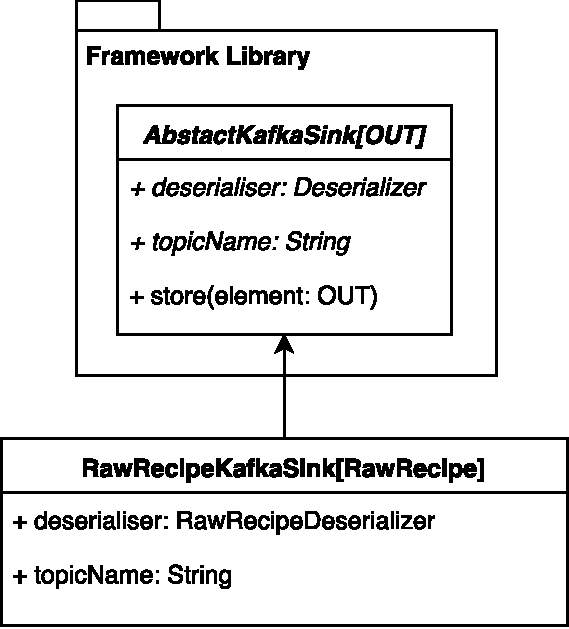
\includegraphics[width=0.3\textwidth]{importer-sink}\\
  \caption{Class diagram of input adapter sink and implementation}
  \label{fig:importer-sink}
\end{figure}

\subsection{Implementation of the adapter component}

As a third component a object must be created that wires up the previous two components, this means to combine the data source, the UDF and the typed data sink as one entire processing pipeline. For this a runnable object is created inheriting the class \textit{AbstractImporterAdapter}. The class diagram can be seen in figure \ref{fig:import-adapter}.  

\begin{figure}[htb]
  \centering
  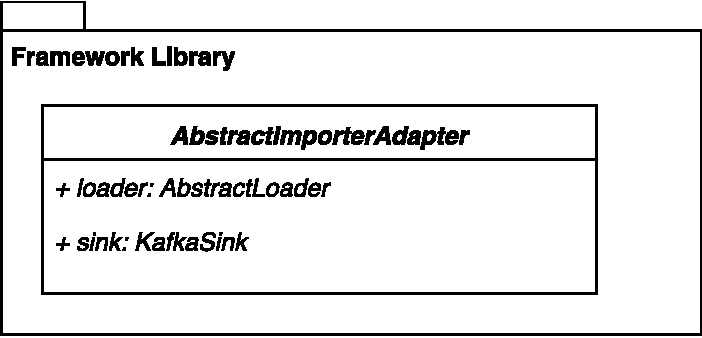
\includegraphics[width=0.4\textwidth]{import-adapter}\\
  \caption{Class diagram of input adapter sink and implementation}
  \label{fig:import-adapter}
\end{figure}

\subsection{Evaluation on library on recipe example}
The library for the import adapter is tested and showcased on the example of two sources of recipes. One source is a MongoDB collection \footnote{A collection in a MongoDB is equal to a table in a SQL database and contains a certain type of entities, named documents.}, the other source is a CSV file. Both sources contain recipes in a different schema. Therefor the input adapter library needed to be extend by a CSV loader (equal to the MongoDB source explained in section \ref{ssec:loadercomponent}). Concrete implementations of the both schemas as well s the raw recipe format are made and require very low programming work. The concrete implementation of the KafkaSink only needs to provide a serializer for the common raw recipe. The utilization of the play-json library reduced the work to a minimum. The final importer job for both sources is a minimalistic implementation combining respectively the source and the common raw recipe Kafka sink.

\section{Implementation of the transformation pipeline}

The concept of the transformation pipeline suggests a component that can apply several transformation functions on raw entities of a deterministic schema.

\subsection{Implementation of the common functionality}

The container framework Akka streams already provides a wide toolset of functionalities for data stream processing. As of the strong customization of the transformation step a less generic approach is chosen compared with the input adapters. 
\\\\
The main common component for the transformation pipeline are the input and output interfaces. Unifying the framework to one common data transportation layer and the concept of raw formats enables the reuse of components of the input adapters. Similar to the concept of the loader in the previous section a Kafka source is is implemented as part of the library for the transformation pipeline. The Kafka source is generic in that way that it is able to load any entity from a Kafka topic. The concrete implementation must then only provide a deserializer\footnote{A deserializer is a component, that defines how a class and its attributes are written to a specific output format.} and the name of the topic.
\\\\
The component writing the the source, again Kafka, can be taken from the input adapter library classes. As outlined above, it is an generic implementation, that is able to write any object to a Kafka topic by providing a deserializer and the topic name.

\subsection{Implementation of transformation pipeline steps}

Having the source and sink for the transformation pipeline provided by the library, the connection transformation steps can be introduced. For the realization of the stepwise approach we take advantage of the toolset of Akka streams. The concepts in chapter \ref{cha:chapter4} already explains idea of UDFs and the usage for the transformation pipeline. Mainly two functions of Akka streams are necessary to build the required pipeline. Those are \textit{map(.)} and \textit{mapAsync(.)}. The implementation of the pipeline is based on a concatenation of those two function where each step takes the element to transform, performs transformation on it and finally returns an modified or updated version of it. \textit{mapAsync(.)} has the additional benefit to call an external blocking resource without blocking the entire transformation pipeline. 
\\\\
A concrete implementation example that deals with \textit{RawRecipes} and transforming them to \textit{recipes} is presented in the listening below it shows the transformation pipeline containing steps for processing and parsing ingredients, instructions and image urls. The source code of the individual functions is due to unimportance not listed here.

\begin{lstlisting}[style=myScalastyle,label={lst:pipeline}]
val rawRecipeSource = KafkaRawRecipeSource("raw-recipes")
val recipeSink = KafakRecipeSink("recipes")

rawRecipeSource
  .map(ingredientService.processIngredients)
  .mapAsync(ingredientService.mapIngredients(_, 4, "de"))
  .map(processInstructions)
  .map(processServes)
  .map(createRecipe)
  .to(recipeSink)
\end{lstlisting}

\textbf{Regular expressions}
The degree of automation of the feature extraction pipeline can be controlled by the effectiveness of applied transformation and parsing functions. Simple errors and deviations within the raw entity can be captured with simple regular expressions. Such a processing step is applied by calling \textit{ingredientService.processServes}. It uses regular expressions that separate the field \textit{"amount unit"}. In this case a very deterministic input can be expected. Hence a simple expression that matches on a combination of numbers and alphanumeric characters separated by zero or more spaces. The capturing groups\footnote{A capturing group is a group of regular expressions that capture the text matched within that group as a unit.} for amount and unit enable a deterministic separation of both attributes for a given ingredient.
\\\\
\textbf{Self learning systems}
As defined in the concept, the framework for feature extraction must also be able to learn from its input. This core requirement can easily applied in a further transformation function and the degree of learning defined by the implementing instance. An approach taken at the reference implementation of food recipes utilizes a fulltext search engine and a continuous update of a learning data set for increasing learning rate over time. 
\\\\
The implemented example of the framework uses Elasticsearch to overcome the varying manifestations of ingredient names on recipes. Elasticsearch is a search engine based on the Apache Lucene project. The search engine supports fulltext search on schema-free JSON denouements powered by inverted indices\footnote{A inverted index is a lookup table where all possible manifestations are listed and point to the documents in which they are contained.}. The idea is to find find the universal ingredient name by searching such with the raw ingredient string from the data source. A fuzzy\footnote{A fuzzy search on Elasticsearch finds all possible matches within a maximum edit distance.} search based on n-grams\footnote{A n-gram is a continuous sequence of substrings of length n of a underlying longer string (e.g. "reci", "ecip", "cipe" are all possible 4-grams for the string "recipe").} returns possible mappings of the raw ingredient string to universal ingredient name. 
\\\\
For example the string "Paprika, rot" will match the following universal ingredient names:
\begin{enumerate}
\item rote Paprika
\item Paprika
\item edelsüßes Paprikapulver
\end{enumerate}
This mapping can be taken and verified in a downstream quality assurance check. After a positive feedback the raw ingredient string (here "Paprika, rot") is stored with the ingredient Paprika. Over time the data set contains several manifestations of one ingredient and enables better and more accurate search results. Over the long term systems knowledge base is a list of ingredient documents containing the universal name and possible different wordings for each ingredient. The performance of the system is discussed in chapter \ref{cha:chapter6}

\textbf{Machine learning models}


\section{Implementation of output adapter}

The concept from section \ref{sec:componentsoutput} defined a toolset based component that provides the possibility of combining several output formats. Figure \ref{fig:output-adapter} illustrates three different output adapters:
\begin{itemize}
\item Feature Extractor
\item JSON Serializer
\item Log Appender
\end{itemize}

\begin{figure}[htb]
  \centering
  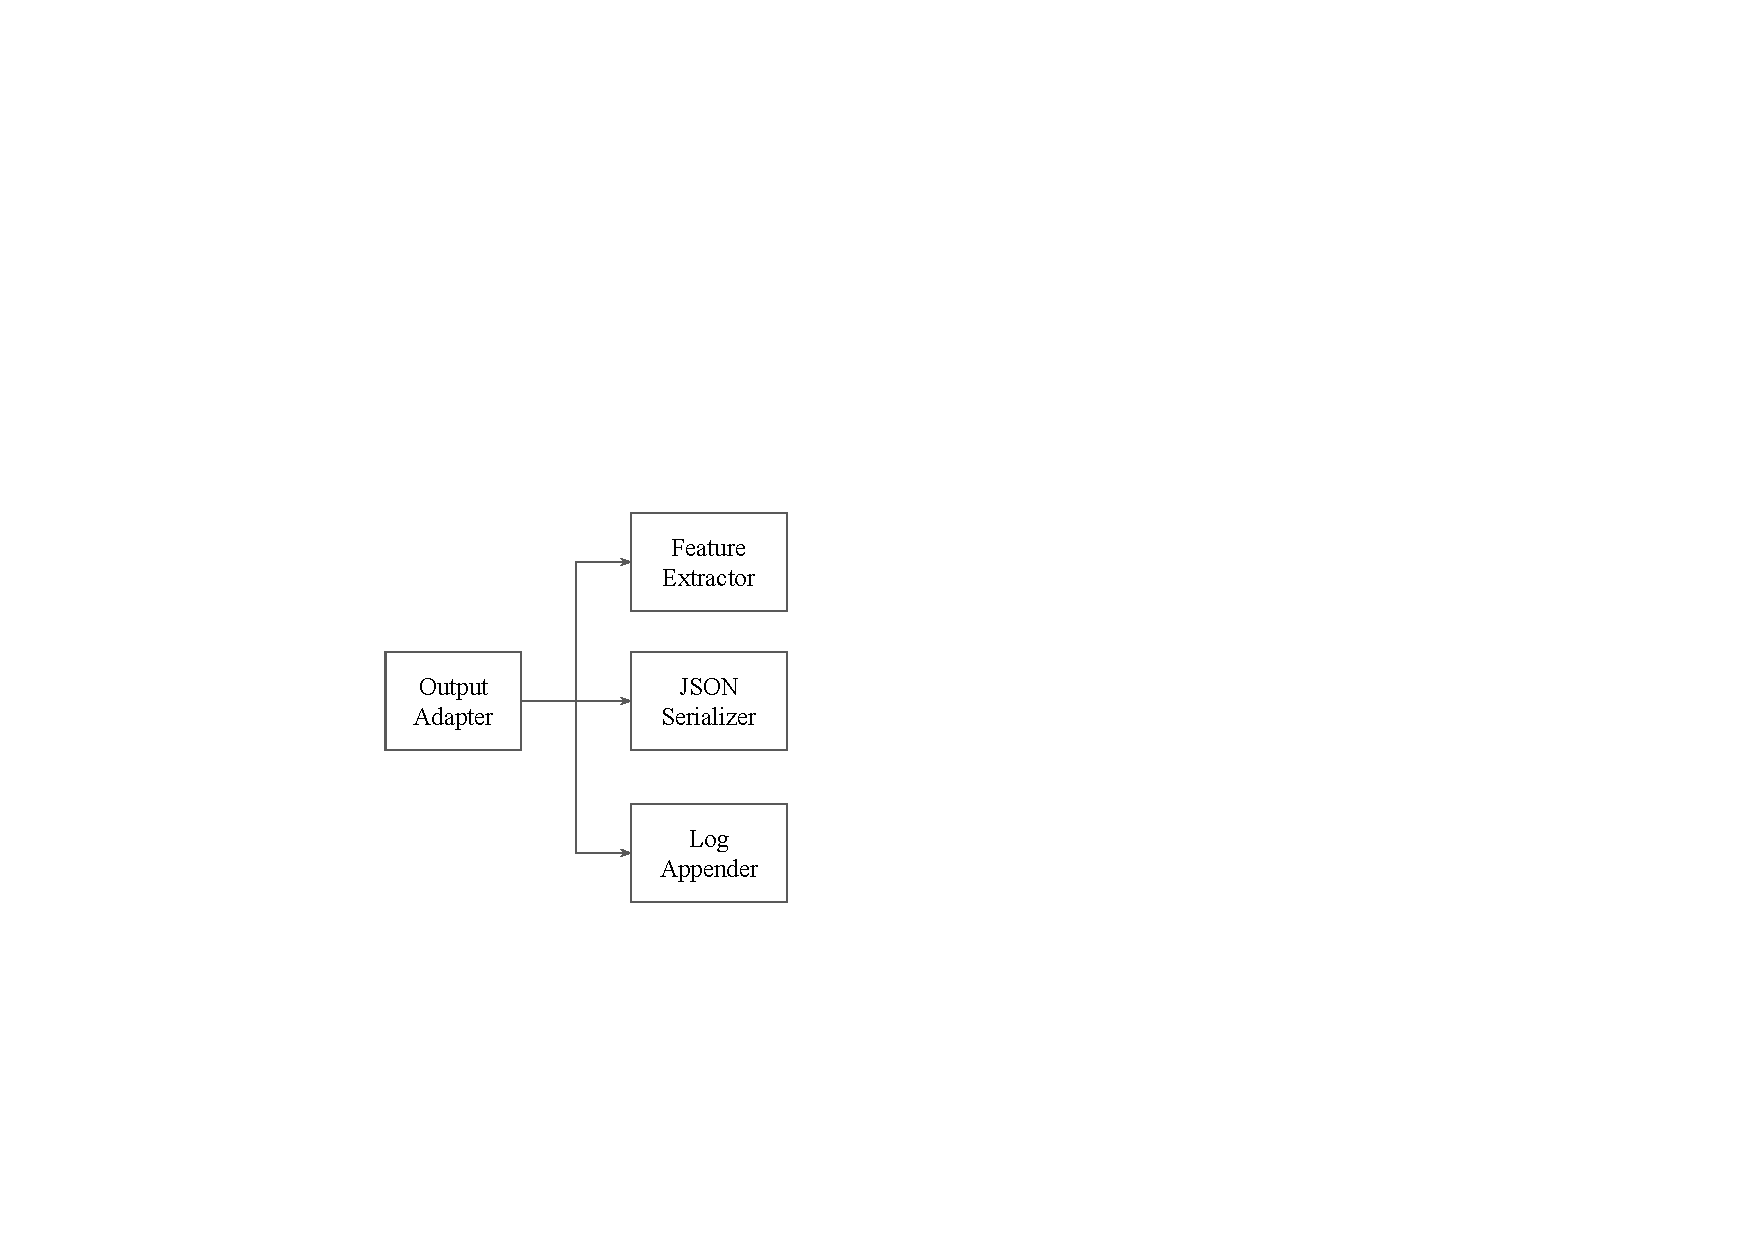
\includegraphics[width=0.4\textwidth]{output-adapter}\\
  \caption{Overview of message flow in the output adapter}
  \label{fig:output-adapter}
\end{figure}

The most impotent for a framework for automated feature extraction is clearly the Feature Extractor. The two further examples are serve the visualization purpose. In the proof of concept implementation the JSON Serializer Adapter is used for deliver the homogenized data for a quality assurance fronted. The Log appender is used for streaming the processed data into a standardized logging system, such as Logstash. Logstash is processing pipeline for bundling logs.
\\\\
The overall adaptability was achieved by the Akka stream API. Akka stream provides the ability of defining data streams, combining and splitting them. For the output adapter the latter was used. Via simple DSL\footnote{Domain-specific language is a abstraction of a programming language for a specific domain} for creating flow graphs of Akka streams. The listening \ref{lst:output} below. shows a reference implementation. The DSL of Akka streams is very intuitive and perfectly suitable for such a use case. It causes low programming overhead and promises fast exchange and extension of the adapter component. The source is again a Akka stream source reading from the underlying transportation layer. \textit{RecipeKafkaSource} again, only has do define the deserializer for the specific entity and the Kafka topic of recipes.

\begin{lstlisting}[style=myScalastyle,label={lst:output}]
val in = RecipeKafkaSource()
val featureExtractorSink = RecipeFeatureExtractorSink()
val jsonSink = JsonSink[Recipe]()
val logAppenderSink = LogAppenderSink[Recipe]()
val adapter = builder.add(Broadcast[Recipe](3))

in ~> adapter ~> featureExtractorSink
adapter ~> jsonSink
adapter ~> logAppenderSink
\end{lstlisting}

The \textit{RecipeFeatureExtractorSink} finally creates feature vectors from a cleaned and stable recipe information entity. It is up to the demand of the developer which features are extracted. As feature engineering is not part of this work, details are not discussed here. The literature provides several approaches and ideas about feature engineering. 
\\\\
For the reference implementation binary features of the recipe ingredients were extracted. A binary feature vector is a vector only containing zeros and ones. If a specific attribute is present in the entity to represent, the corresponding field is set to one, otherwise zero. From an implementation aspect, the unified ingredient names where hashed to determine the the index within the the feature vector. This approach is reliable, as first, the possible manifestations of ingredients is finite, and second, the used hashing algorithm, here murmur-hash, returns a deterministic hash for each possible string.

\begin{figure}[htb]
  \centering
  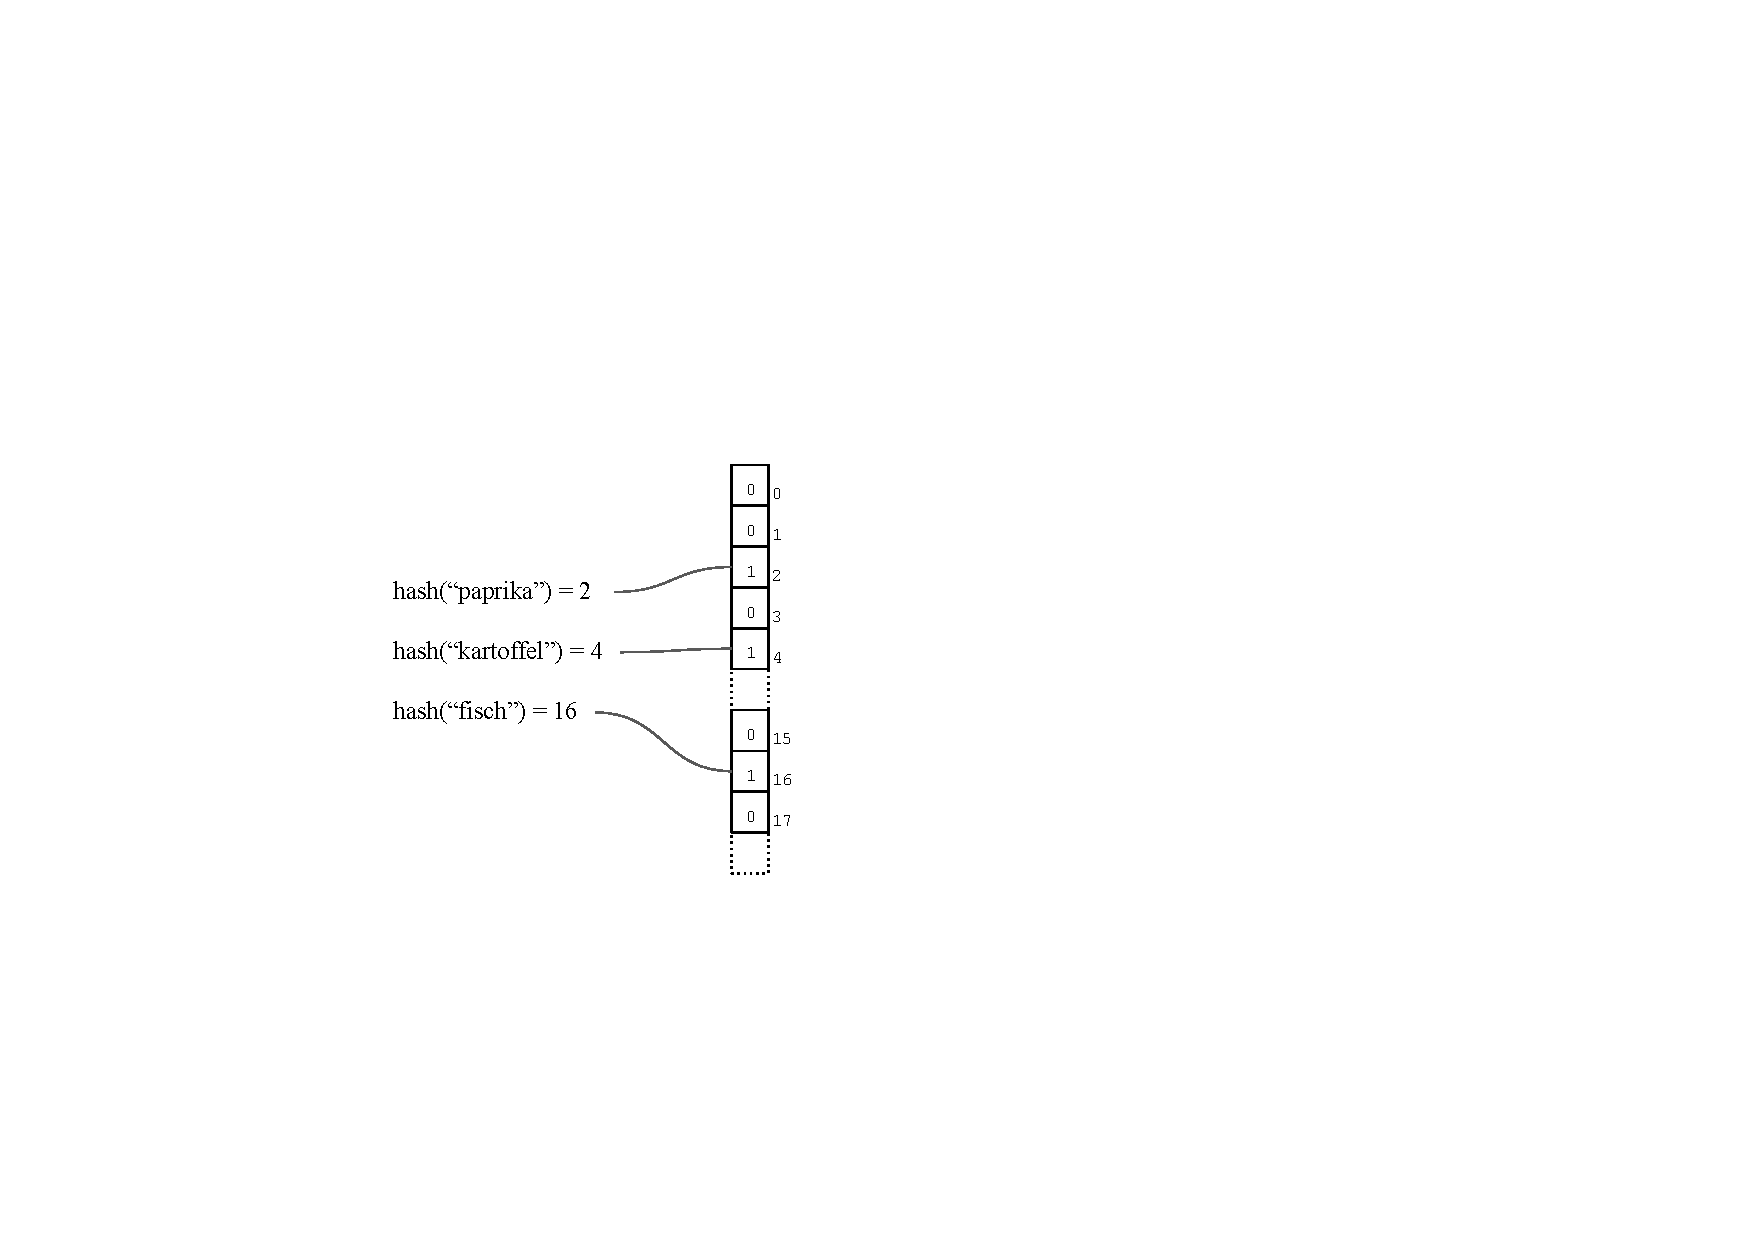
\includegraphics[width=0.4\textwidth]{bin-feature}\\
  \caption{Binary feature vector for the ingredients: paprika, kartoffel and fisch}
  \label{fig:bin-feature}
\end{figure}

Concluding it can be said, that the choice of the underlying container framework Akka stream as well as the programming language Scala plays well together with the domain of automated data processing. The available libraries and custom libraries reduced the implementation overhead for a processing pipeline for unification of semi-structured data. The idea of an additional abstraction layer on top of the data transfer component, Kafka and the Akka stream framework enables a simple adaption of the concrete framework implementation for different sources, entities and domains. The work is reused for the set up of a feature extraction pipelines for food products.